\documentclass[review]{cvpr}
% \documentclass[final]{cvpr}

\usepackage{times}
\usepackage{epsfig}
\usepackage{graphicx}
\usepackage{graphics}
\usepackage{amsmath}
\usepackage{amssymb}
\usepackage{listings}

% Include other packages here, before hyperref.
\usepackage{multirow, multicol, booktabs}
\usepackage{caption}
\usepackage{subcaption}
\usepackage{tabularx}
% If you comment hyperref and then uncomment it, you should delete
% egpaper.aux before re-running latex.  (Or just hit 'q' on the first latex
% run, let it finish, and you should be clear).
\usepackage[pagebackref=true,breaklinks=true,colorlinks,bookmarks=false]{hyperref}


\def\cvprPaperID{****} % *** Enter the CVPR Paper ID here
\def\confYear{CVPR 2021}
% \setcounter{page}{4321} % For final version only


\begin{document}

%%%%%%%%% TITLE
\title{Breast Cancer Histopathological Images Segmentation and Classification using Vision Transformer}
\author{Bedionita Soro (20205677), Ying Hui Tan (20204871), Oh Joon Kwon (20213044)}

\maketitle

\begin{abstract}
Breast cancer is one of the wide-spread diseases in the world. Its detection at an early stage is crucial for increasing the chance of successful treatment of patients. However, pathologists often need to scan a large set of Whole Slide Images (WSIs) to identify the regions and the type of tissues, which is laborious task. There have been several deep learning based approaches to reduce the burden. Previous approaches made use of convolutional neural networks (CNNs) as feature extractor, which often struggle to generalize in different domains. Moreover, these approaches often takes sophisticated post-processing techniques and relies on patch-based technique treating each patch as an image. In this paper, we propose an end-to-end method that exploits the expressive capacity of Vision Transformer (ViT) and its variants. Our method can be put into three main phases. First, we build a classification model for breast cancer diagnosis. Second, we design a ViT based segmentation model for WSIs. Finally, we investigate the combination of these models for domain adaptation in other types of tissue segmentation. The preliminary experiment on BreakHis dataset has demonstrated the proposed method efficiently competes with the existing state-of-the-art results.
\end{abstract}

\section{Introduction}
Breast cancer \cite{7312934} is one of the most wide spread types of cancer whose detection and categorization is not straightforward even for expert pathologists \cite{Randell01}. In fact, pathologists have to scan a large set of Whole Slide Images (WSI), which can be in the order of gigapixels to localize the regions of tumor as well as to identify the type of tumor. To ensure that there is no malpractice, this has to be done in several magnification levels\cite{KRUPINSKI20061543}. Fortunately, due to recent advancements in deep learning specifically in pattern recognition\cite{russakovsky2015imagenet}, there has been a growing interest in applying deep learning to tissue segmentation and breast cancer classification using WSI\cite{lei2020medical,SRINIDHI2021101813}. 

However, WSI are very large to segment with current deep learning methods without reducing the images' dimensions. Even though reducing the image size may have little effects on the cancer classification task (benign and malignant), detecting the region of interest through tissue type segmentation requires that images not be resized. To overcome such limitation, patch-based methods have been introduced\cite{7780635} for both tissues semantic segmentation and cancer classification. The patch-based methods consist of dividing WSI and ground-truth segmentation mask into small chunks of images. Patch-based approaches have been broadly investigated\cite{8451551} and are actually commonly used in large scale medical image segmentation. The extracted patches can be saved on the disk, but this can become impractical given the number of the images. Another challenge is that some patches do not have distinctive features and may require a good post-processing to achieve a desired outcome. Moreover, patches are treated independently without much regard to their global relationship in the whole image.

In this paper, we propose a new approach that exploits the current state-of-the-art Vision Transformer architecture to take advantage of WSI at once by considering each image as a sequence of patch tokens. Such an approach is fast to train for both cancer types classification and tissues type semantic segmentation with less effort in preprocessing and post-processing. Although similar architecture has been introduced in other medical images segmentation related work \cite{chen2021transunet}, to our knowledge, this is the first time this method is applied to WSI for breast cancer images segmentation and tissue classification. In most existing related work where Vision Transformer is used have been to exploit its pretrained feature extraction capability. We consider a similar approach as machine translation when dealing with semantic segmentation, where a sequence of images is given as input to produce a sequence of segmented masks.

The work of this paper can be divided into three parts. First, we propose Vision Transformer model for breast cancer classification. Second, we use similar base architecture for tissue type segmentation. Finally, we use the semantic segmentation model as feature extractor for cancer classification and investigate further domain adaptation. The contribution and the novelty of this paper are summarized as follows:
\begin{itemize}
    \item We propose the first Vision Transformer based cancer tissues segmentation and cancer types classification using WSI of breast. To our best knowledge, this approach has not yet been applied to WSI  and for large scale image segmentation and classification. 
    \item The proposed method require less postprocessing compared to the existing patch-based approaches.
    \item The proposed method is fast to train and achieve competitive results compared to existing complex convolution neural network model on classification tasks.
\end{itemize}


\section{Related work}
\noindent \textbf{WSI Classification.} Using WSI is one of the best ways to integrate deep learning in cancer diagnosis, specifically for breast cancer. In breast cancer diagnosis, the classification can be binary (benign or malignant) or multiclass. Hameed et al \cite{s20164373} used an ensemble of deep learning model such VGG16 and VGG19 to design a classifier model for non-carcinoma and carcinoma breast cancer histopathology images identification. However, this model is hard to train due to the complexity of VGG network. In the same vein of binary classification, Abdullah-Al  Nahid et al. \cite{2362108} employed CNN and LSTM among other features extraction methods to design a model that can accurately classify cancer type, benign or malignant. Similar approach has been proposed in \cite{alom2018breast} where they exploited the Inception recurrent CNN architecture to improve the performance on BreakHis dataset\cite{BENHAMMOU20209}.

On the other hand, some studies included the sub-classes of cancer in a multiclass classification approach \cite{Han2017}. \cite{9218931} proposed a comparison study of several deep learning approaches for breast cancer classification. Furthermore, \cite{BENHAMMOU20209} conducted a survey where they provided a performance analysis of existing state-of-the-art methods on BreakHis dataset. \cite{10.1371/journal.pone.0214587} is one of these best approaches for binary classification. They inserted squeeze and excitation module to a ResNet model and adjusted the optimization parameters to increase the classification performance. The existing methods are mostly based on patch-based approach where the challenges arise. One of the challenges is to distinguish informative patches from non-informative patches. It is also challenging to classify an image based on several sequences of patches. Additionally, dividing large images into patches and save to disk will triple the memory requirement (original, patches, and online execution). Our approach leverages all these challenges of existing method and can achieve competitive results. With the transformer architectures, we are still using patch-based approach but this method can take variable length of patches while extracting relevant image features with attention mechanism.\\
\\
\textbf{WSI Segmentation.} There is a large body of work on WSI segmentation\cite{vu2018methods}. Most recent works on WSI segmentation focus on deep learning\cite{10.3389/fmed.2019.00264}. However, applying deep learning for WSI segmentation is a challenging task because of the large size of the images where resizing is not generally recommended for accuracy. Therefore, most existing deep learning approaches exploit patch-based based segmentation\cite{PRIEGOTORRES2020113387, Fu_2018}. In \cite{10.1117/12.2581229}, active learning was used to enhance the performance of patch based WSIs segmentation. Similarly in \cite{Xulargescale2017}, pretrained deep convolutional neural network (CNN) was used to improve the performance of patch-based segmentation of brain WSIs for tumor detection. To investigate the deep learning model generalization, Mahendra Khened et al.\cite{khened2020generalized} proposed a deep learning framework for histological tissue segmentation. In their study, they explored different datasets including a breast cancer WSI dataset and evaluated the model's uncertainty and generalization performance against distributional shift. 

Moreover, several studies such as \cite{Guofast2020} exclusively studies breast cancer WSI segmentation. In addition to WSI segmentation for cancer or disease detection, deep learning methods are being used for cancer classification from WSI\cite{XU2014591}, specifically for the  breast cancer. Most existing WSI segmentation methods are patch-based, therefore they require more additional post processing processing to combine the patches. Furthermore, some patches can be non-informative. Those methods commonly use deep CNN architectures which can slow the training process and difficult to train on computation resource limited devices. Transformer architectures can extract meaningful features from natural images. \\
\\
\textbf{Transformer.} Transformer architecture was first proposed by Vaswani et al.\cite{vaswani2017attention}. The essence of the architecture lies in the multi-headed self-attention (MHA) mechanism to learn the relationships among sequential tokens. MHA can be expressed as the following
\begin{equation}
\begin{split}
    \text{MHA}(Q, K,&\, V) =  \text{Concat}(A_1, \dots, A_h)W^O, \\[3mm]
    \text{where } A_i & := \text{Attention}(QW_i^Q, KW_i^K, VW_i^V) \\
        & = \text{softmax} \left( \frac{(QW_i^Q)(KW_i^K)^\top}{\sqrt{d_k}} \right) VW_i^V,
    \label{attention}
\end{split}
\end{equation}
where $Q, K, V$ are input query, key, value vectors, $W_i^Q, W_i^K \in \mathbb{R}^{d_{\text{model}}, d_k}, W_i^V \in \mathbb{R}^{d_{\text{model}}, d_v}$ are trainable query, key, value weights at the $i$-th attention head, $d_{\text{model}}$ the model dimension , $h$ number of heads, $d_k, d_v$ key and value dimension. By only using self-attention for processing sequential data, Transformer has shown state-of-the-art performance in numerous natural language processing tasks such as machine translation and sequence generation. Since its conception, Transformer architecture has been adapted to other domains.\\
\\
\textbf{Vision Transformer} Vision Transformer (ViT)\cite{dosovitskiy2020image} closely adapts Transformer Architecture from natural language processing for image classification. The concept consists of dividing the whole image into small chunks analogous to the sequence of language tokens. There are a few modifications from the original Transformer architecture for image domains:
\begin{enumerate}
    \item In order to circumvent the quadratic memory bottleneck, ViT takes in patches of images instead of pixels that are flattened then embedded via linear layer, essentially taking patches as tokens.
    \item Because of the sequential nature, ViT can take higher resolution inputs. However, position embeddings need to be interpolated for finetuning. This has been shown to be emprically effective in the subsequent downstream tasks. 
    \item As in the pretrained language model BERT, a classification token is appended before the patch tokens.
\end{enumerate}
Through extensive experiments, it has been proved that the ViT outperforms the existing state-of-the-art models in image classification tasks, thereby several variants of ViT have been proposed\cite{wu2021cvt,zhou2021deepvit}. Furthermore, ViT model can be a good feature extractor or encoder given that it has been trained on various type of datasets. Therefore, we apply this promising architecture to histological images segmentation and breast cancer classification.

% \begin{table}[ht]
%     \centering
%     \begin{tabular}{cccc}
%         \toprule
%         Models & Image size & \# Params & FLOPs  \\ \midrule
%         \multicolumn{4}{c}{Convolution} \\ \midrule
%         Resnet-101 & $224^2$ & 45M & \\
%         EffNet-B3 & $300^2$ & 12M & 1.8G \\
%         EffNet-B4 & $380^2$ & 19M & 4.2G \\ \midrule
%         \multicolumn{4}{c}{Transformers} \\ \midrule
%         ViT-B/16 & $384^2$ & 86M & 55.4G \\
%         ViT-L/16 & $384^2$ & 307M & 190.7G \\
%         DeiT-B   & $224^2$ & 22M & 4.6G \\
%         DeiT-B   & $384^2$ & 86M & 17.5G \\ \bottomrule
%     \end{tabular}
%     \caption{Computation and parameter comparison of different image model backbones on ImageNet. The table was adapted from \cite{touvron2021training}.}
%     \label{computation_comparison}
% \end{table}


\section{Method}
\begin{figure}[ht]
\begin{center}
% \fbox{\rule{0pt}{2in} \rule{0.9\linewidth}{0pt}}
   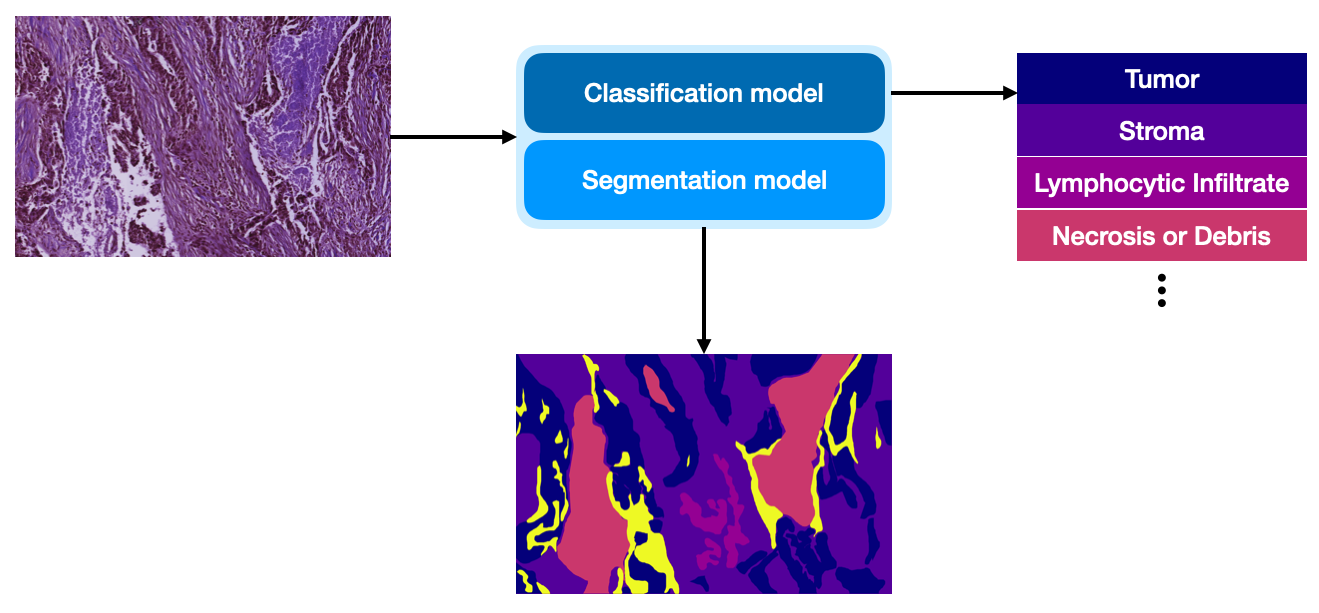
\includegraphics[width=0.8\linewidth]{media/roi1-new.png}
\end{center}
   \caption{Block diagram of the model for WSIs segmentation and classification}
\label{fig:roi}
% \label{fig:onecol}
\end{figure}
Figure \ref{fig:roi} depicts the block diagram of the proposed method. Our approach can be decomposed into two main steps: first, we build a classification model based on ViT for breast cancer detection, then we build a model for WSI segmentation. We then combine those models to produce a multi tasks model. Another option we have is to apply domain adaptation to another organ segmentation dataset. 
\subsection{Classification}
\begin{figure}[ht]
\begin{center}
% \fbox{\rule{0pt}{2in} \rule{0.9\linewidth}{0pt}}
   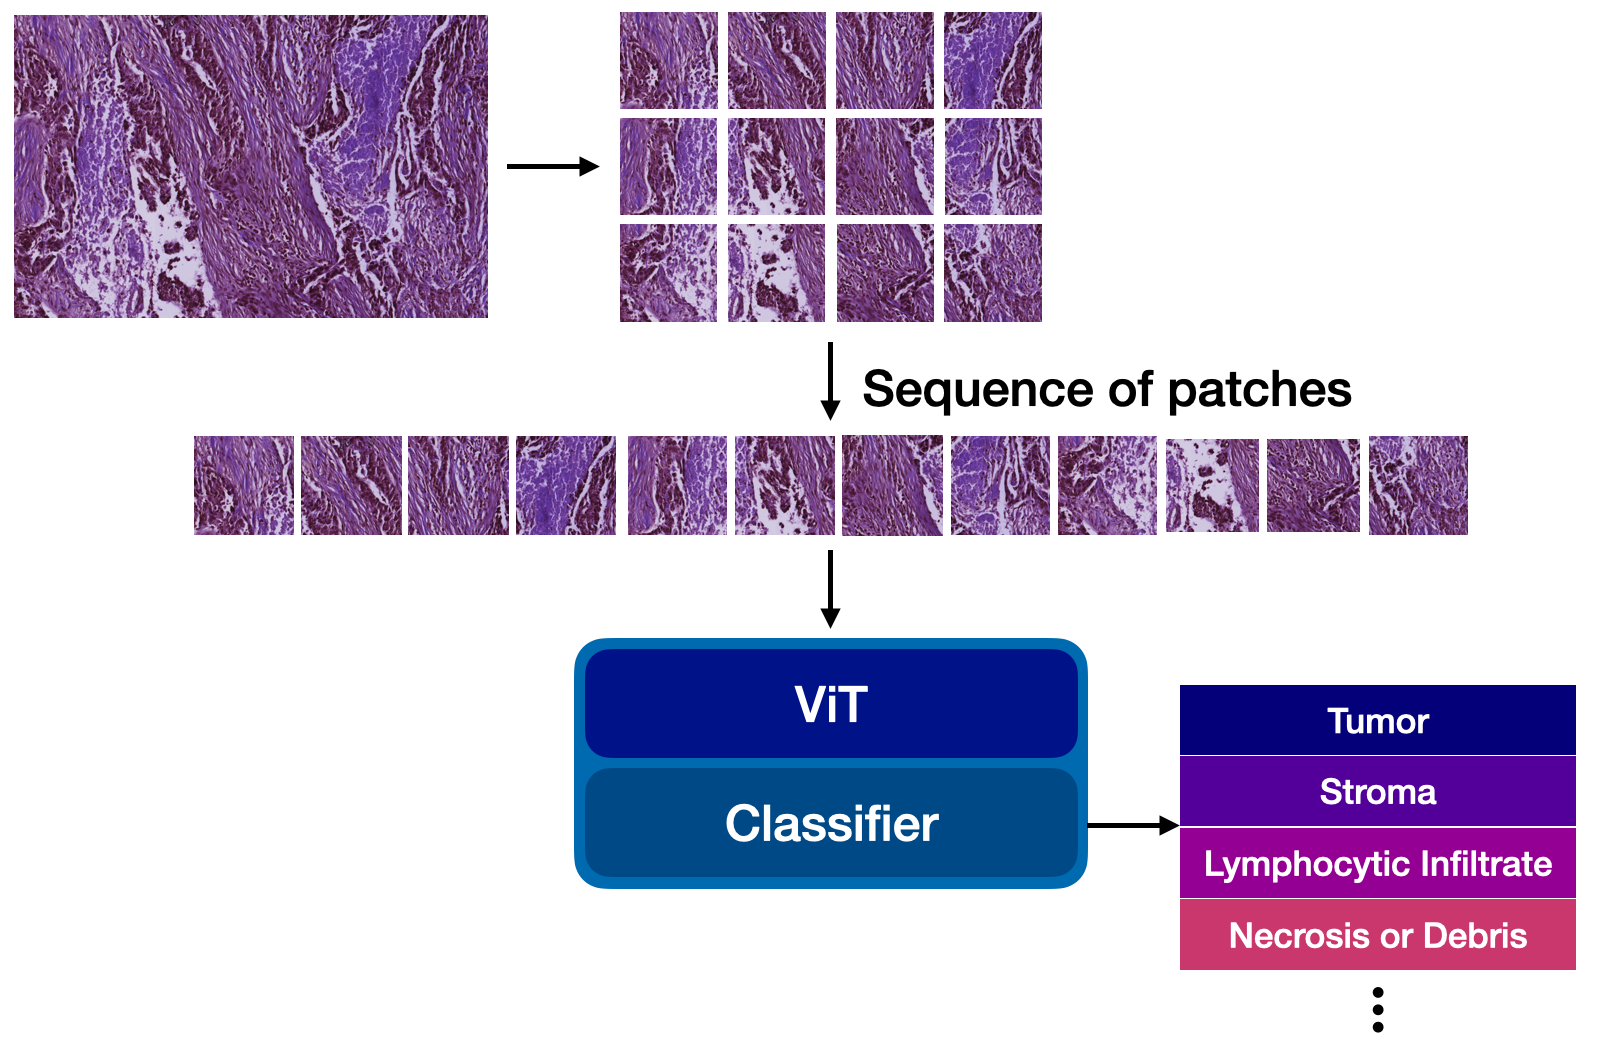
\includegraphics[width=0.8\linewidth]{media/classify-new.png}
\end{center}
   \caption{Block diagram of the model for WSI classification}
\label{fig:cls}
% \label{fig:onecol}
\end{figure}
In this section we begin with the classification model. Our first goal is to use the ViT to accurately predict the class of breast cancer given a whole slide image as input. Previous works \cite{7780635} decompose the images into patches then fit those discriminative and non discriminative patches to a CNN one by one or resize to a lower resolution. We resize to an appropriate resolution (not necessarily lower for CNN) then use all patches of each image at once with ViT. Given an image $X^{H \times W \times C}$ with spatial resolution ${H \times W}$, ViT firstly divides it into $N = \frac{HW}{P^2}$ patches where $P$ is the patch size. This leads to each spatial dimension being a multiple of patch size. However, WSI do not always come in such manner. To deal with the design choice we propose to use rectangular patch size and also use padding strategy in case the sizes do not match. Although padding may have small effect on classification results, it is important for WSI segmentation. The new number of patches can be computed as in \ref{npatch}:
\begin{equation}
    N= \left\lceil\frac{H}{P_1}\right\rceil \cdot \left\lceil\frac{W}{P_2}\right\rceil,
    \label{npatch}
\end{equation}
where $P_1$ and $P_2$ are the spatial dimensions of a patch. Figure \ref{fig:cls} depicts the proposed architecture for cancer WSI classification.

\subsection{Segmentation}
\begin{figure}[h]
    \centering
    \begin{subfigure}{0.5\textwidth}
        \centering
        \resizebox{0.8\columnwidth}{!}{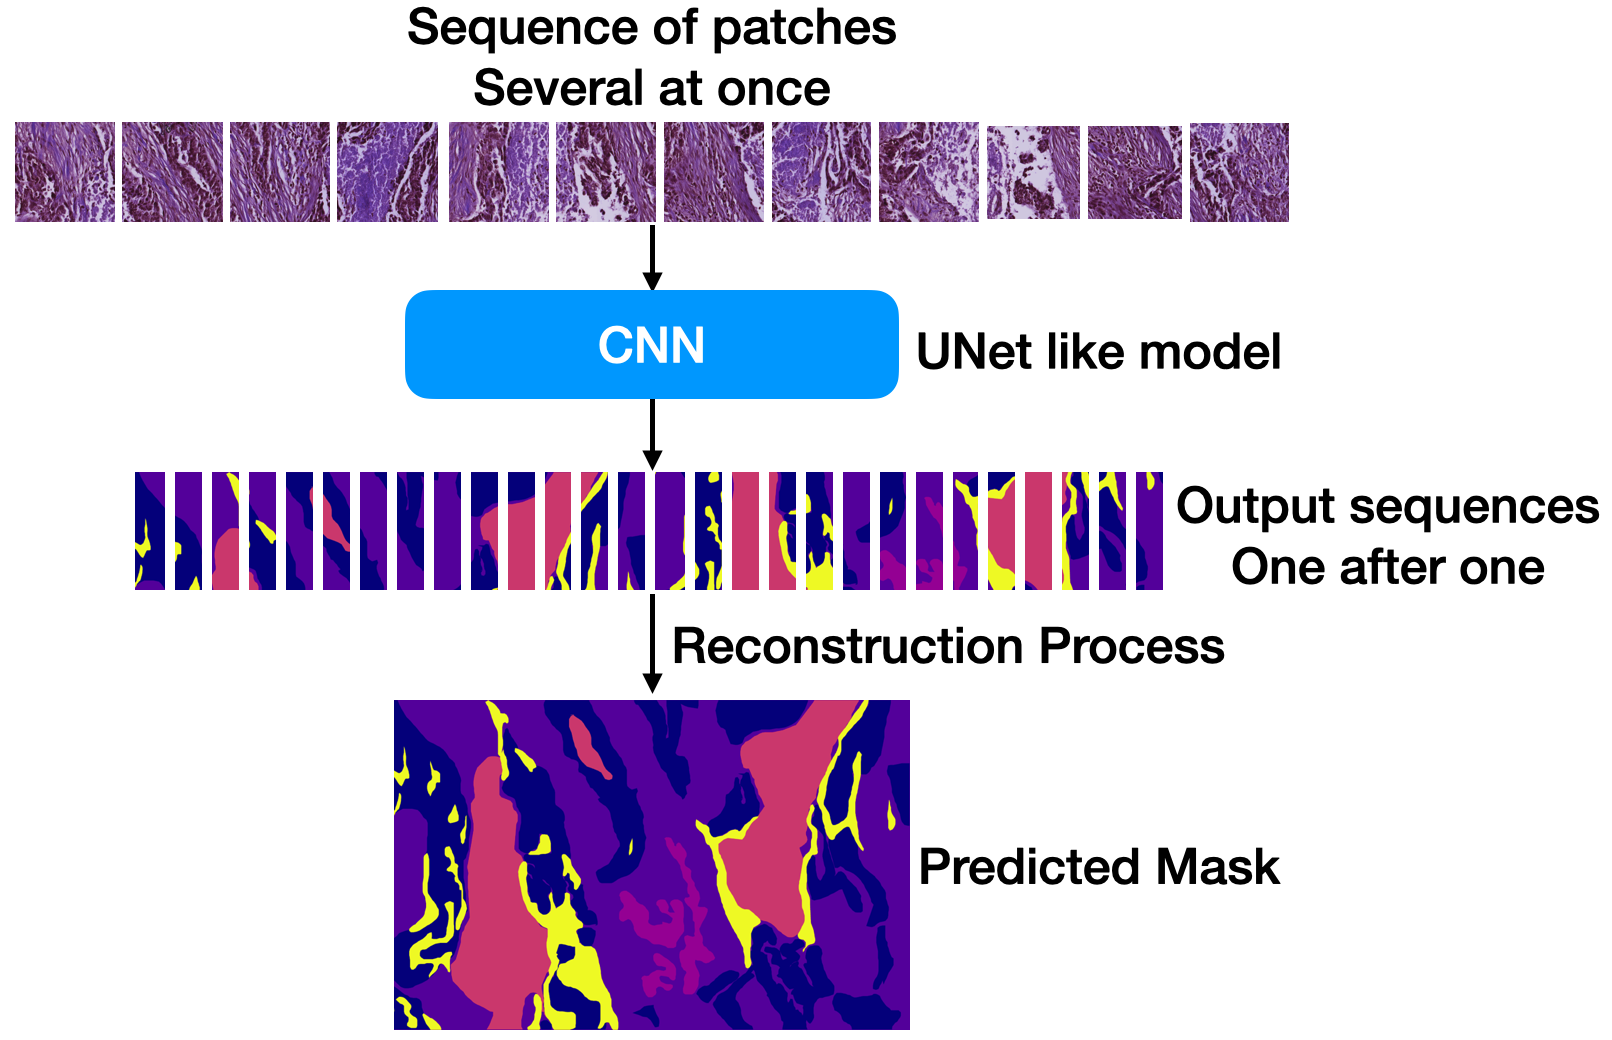
\includegraphics[width=0.8\linewidth]{media/prev-new.png}}
        \caption{Previous patch-based approach}
        \label{fig:prev}
    \end{subfigure}
    \begin{subfigure}{0.5\textwidth}
        \centering
        \resizebox{0.8\columnwidth}{!}{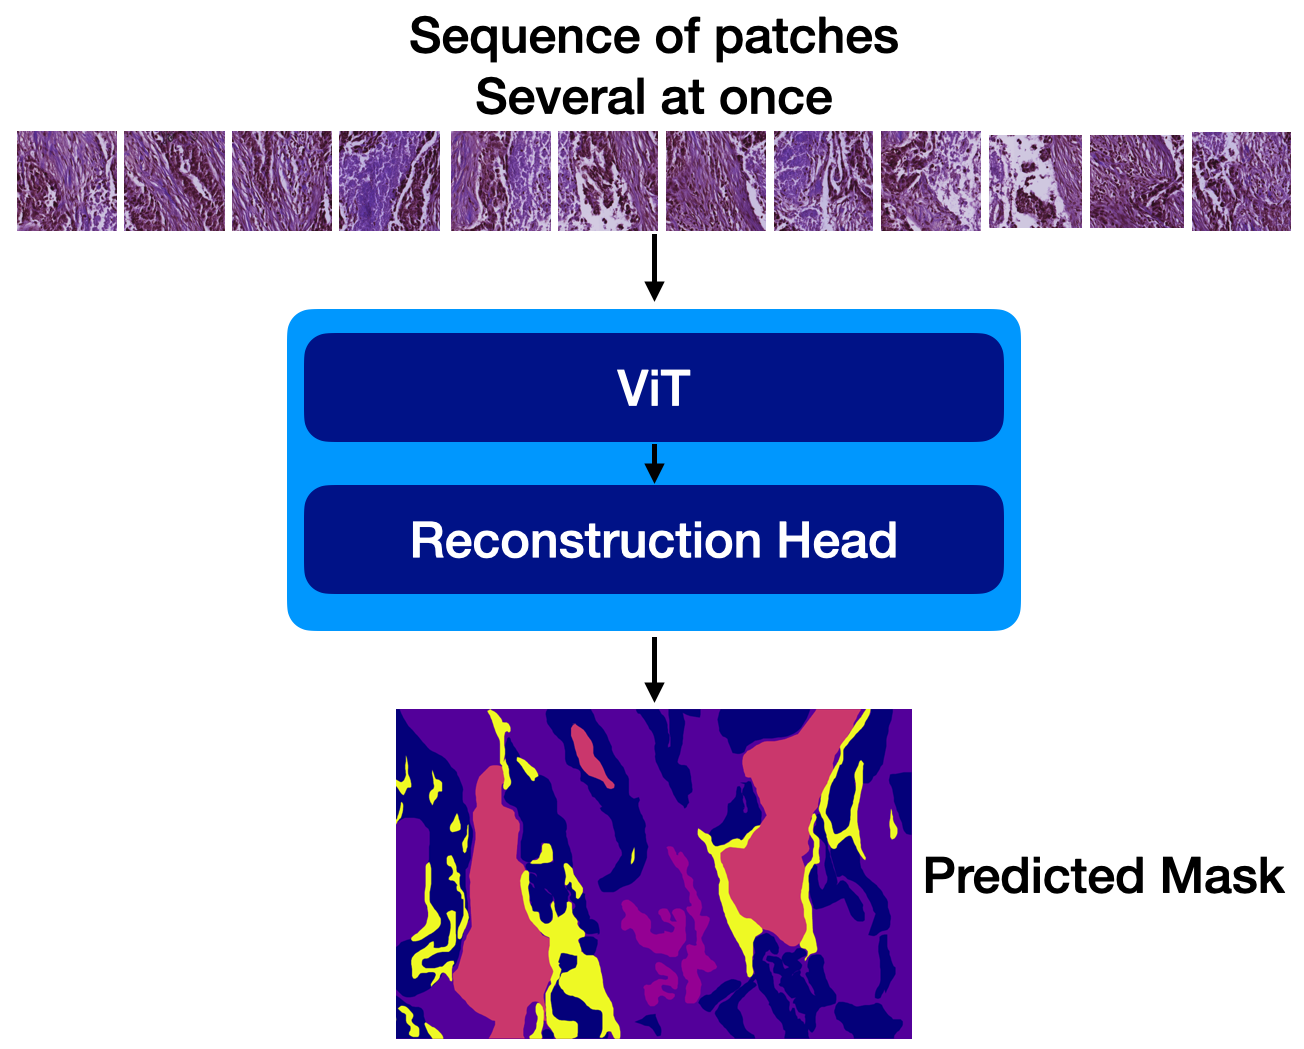
\includegraphics[width=0.8\linewidth]{media/prop-new.png}}
        \caption{Proposed segmentation architecture}
        \label{fig:prop}
    \end{subfigure}
\caption{WSI segmentation model diagram}
\label{fig:seg}
\end{figure}

If the image is too large we divide it into chunks of appropriate size then use those chunk as original image. Doing so we reduce the number on chunks to be treated sequentially compared to existing approaches which will produce large number of chunks then treats them sequentially \ref{fig:prev}. Most existing biomedical images segmentation approaches integrate UNet\cite{ronneberger2015unet} or a large CNN backbone that can only take fixed input sizes. Our method also have the advantage to allow the insertion of part of an UNet module at the output of the transformer if needed.

Figure \ref{fig:prop} depicts the proposed segmentation approach. The model can produce a sequence of images at once if the ground true is a sequence of images like in machine translation. Also, we can bypass the post processing part and produce accurate segmentation mask. The reconstruction head in the Figure \ref{fig:prop} can be a set of convolution layers to produce the appropriate final shape for the output model. \\
The input image to our segmentation network is a 2D image of size $(H \times W \times C)$ where $H=W$ are the image height and width, and $C$ the number of channels (3 for RGB images). 

The input image is then partitioned to a sequence of patches of size $(P\times P\times C)$. These patches are passed through the transformer which outputs the embedding matrix of shape $(B, N, d)$,  where $B$ is the batch size, $N$ the number of patches and $d$ the embedding dimension. For reconstructing the prediction mask, we can add a multi-layer perceptron to transform that embedding into a matrix of shape $(B, cHW)$ and reshape to $(B, c, H, W)$ where $c$ is the number of classes. Such an approach requires a lot of memory resources for large images. Another way to reconstruct the segmentation mask is to directly reshape the embedding matrix into $(B, N, d_1, d_2)$ where $d = d_1\times d_2$, then apply transpose convolution as in UNet architecture. This approaches reduces largely the numbers of convolution layers while playing the role of the encoder in UNet-like architecture.


\subsection{Evaluation metric}
To evaluate the proposed method, we use the following metrics for each tasks.

\subsubsection{Classification}
\begin{enumerate}
    \item[\textbullet] Accuracy: a naive multi-class classification metric. 
    \item[\textbullet] F-1 score: given TP, FP, and FN are true positive, false positive, and false negative, F-1 score can be computed as 
    \begin{equation}
         \text{F-1} = \frac{2\text{TP}}{2\text{TP}+\text{FP}+ \text{FN}}
         \label{f1-metric}
    \end{equation}
\end{enumerate}

\subsubsection{Segmentation}
\begin{enumerate}
    \item[\textbullet] Pixel accuracy: a naive pixel-wise accuracy metric. 
    \item[\textbullet] Intersection over Union (IoU/Jaccard): IoU, also known as Jaccard index, can be computed in a similar manner to \ref{f1-metric}, but without the constant:
    \begin{equation}
        \text{Dice} = \frac{\text{TP}}{\text{TP}+\text{FP}+ \text{FN}}
        \label{dice-score-metric}
    \end{equation}
    \item[\textbullet] Dice coefficient (Dice/F-1): Dice coefficient is defined to be the following where $\hat{Y}$ and $Y$ are the predicted region from the model and the ground truth region of input image.
    \begin{equation}
        \text{Dice} (\hat{Y},Y)=2\frac{|\hat{Y} \cap Y|}{|\hat{Y} \cup Y|},
        \label{dice-score}
    \end{equation}
    This is equivalent to F-1 score in the context of segmentation, which can be computed by \ref{f1-metric}.
\end{enumerate}

% \begin{equation}
% \begin{split}
%   \text{F1} & = \frac{2\text{TP}}{2\text{TP}+\text{FP}+ \text{FN}}, \\
%   \text{Sensitivity} & = \frac{TP}{TP+FN}, \\
%   \text{Precision} & = \frac{TP}{TP+FP} ,
%   \label{metric1}
% \end{split}
% \end{equation}

\section{Experiments}
\subsection{Classification}
\subsubsection{Dataset description}
Breast Cancer Histopathological Image Classification (BreakHis) dataset \cite{BENHAMMOU20209} was used to assess the performance. This dataset is composed of 9,109 microscopic images of breast tumor tissue collected from 82 patients using different magnifying factors (40X, 100X, 200X, and 400X). It contains 2,480  benign and 5,429 malignant samples ($700\times 450$ pixels, 3-channel RGB, 8-bit depth in each channel, PNG format). Benign and malignant subtypes \ref{TAB1} are also provided which makes this dataset an good choice for comparing models performance. According to the dataset, there are four histological distinct types of benign breast tumors (B): adenosis (A), fibroadenoma (F), phyllodes tumor (PT), and tubular adenona (TA) and four malignant breast tumors (M): carcinoma (DC), lobular carcinoma (LC), mucinous carcinoma (MC) and papillary carcinoma (PC). 

\begin{table}[ht]
\centering
\resizebox{\columnwidth}{!}{\begin{tabular}{c|c|cccc|c|c} %{llllllll}
\toprule
\multirow{2}{*}{Class} & \multirow{2}{*}{Type} & \multicolumn{4}{c|}{Magnification} & \multirow{2}{*}{Total} & \multirow{2}{*}{Sum} \\
& & 40X & 100X & 200X & 400X & & \\ \midrule
\multirow{4}{*}{B} & A & 114  & 113  & 111  & 106 & 444 & \multirow{4}{*}{2480}  \\
 & F  & 253  & 260  & 264  & 237 & 1014 & \\
 & TA & 109 & 121  & 108  & 115 & 453 & \\
 & PT & 149  & 150  & 140  & 130 & 569 & \\ \midrule
\multirow{4}{*}{M} & DC & 864  & 903  & 896  & 788 & 3451  & \multirow{4}{*}{5429}  \\
 & LC & 156  & 170  & 163  & 137  & 626 & \\
 & MC & 205  & 222  & 196  & 169 & 792 & \\
 & PC & 145  & 142  & 135  & 138 & 560 &  \\ \midrule
\multicolumn{2}{c|}{Total} & 1995 & 2081 & 2013 & 1820 & 7909 & 7909\\
\bottomrule
\end{tabular}}
\caption{BreakHis dataset description}
\label{TAB1}
\end{table}

\subsubsection{Experiment setup}
We consider two approaches to evaluate our model which are magnification specific binary(MSB) classification  and  magnification specific multi classes classification (MSM). For the binary classification, we only consider benign and malignant to be the classes. For multi classes classification, we only consider the subclasses. The results of the experiment for binary classification are showed in Table \ref{result1}. In this experiment, we consider two state-of-the-art methods \cite{Xie2019,8353225} on the same dataset.  Data augmentation techniques were not used. Also, we do not use any pretrained models.

We  train the model for both binary and multi-class classification in a multi-label classification manner. In this experiment we train the proposed model from scratch with patch size $(20 \times 50)$ and input size $(460\times 700 \times 3)$. For comparison, the BreakHis dataset is randomly split into 70\% for training and 30\% for testing for each magnification factor. We only consider the methods that preprocess the dataset in the same manner as we do. Table \ref{result0} presents the experimentation results.

\subsubsection{Result}
The model achieves good performance on the disease classes compared to the subclasses. However, the performance of the subclasses can be improved if they are trained separately. The performance on the subclasses is comparable to existing methods \cite{BENHAMMOU20209,Xie2019}. Based on the results presented in \cite{BENHAMMOU20209}, our approach achieves competitive results \ref{result1} compared to existing breast cancer classification method tested on BreakHis. However, further improvement are still needed for the multilabels classification. Therefore, we will perform further experiments with non combined training, parameter tuning to outperform the state-of-the-art on BreakHis and move to tissues segmentation. The results presented in this paper are preliminary results and the final results may different significantly. 

\begin{table}[ht]
\centering
\resizebox{\columnwidth}{!}{
\begin{tabular}{|l|l|l|l|l|l|} 
\hline
\multirow{2}{*}{\begin{tabular}[c]{@{}l@{}}Classification\end{tabular}} & \multirow{2}{*}{criteria} & \multicolumn{4}{l|}{Magnification}  \\ 
\cline{3-6} &  & 40X   & 100X  & 200X   & 400 \\ 
\hline
\multirow{3}{*}{MSB  } & F-1 micro & 99.00 & 98.00 & 100.00 & 99.00  \\ 
\cline{2-6}& F-1 macro & 98.88 & 97.68 & 99.45  & 99.37\\ 
\cline{2-6}& Acc. & 99.00 & 98.08 & 99.50  & 99.45 \\ 
\hline
\multirow{3}{*}{MSM} & F-1 micro & 89.00    & 90.00   & 90.00     &90.00 \\ 
\cline{2-6} & F-1 macro & 87.10 & 86.99 &86.33    & 88.13         \\ 
\cline{2-6} & Acc.  & 89.48  & 89.76    & 90.23    & 89.74 \\
\hline
\end{tabular}}
\caption{Evaluation results on Breakhis dataset.}
\label{result0}
\end{table}

\begin{table}[ht]
\centering
\resizebox{\columnwidth}{!}{\begin{tabular}{cc|cccc|c}
\toprule
\multirow{2}{*}{Works} & \multirow{2}{*}{Year} & \multicolumn{4}{c|}{Magnification} & \multirow{2}{*}{Mean} \\
 & & 40X & 100X & 200X & 400X & \\ \midrule
\cite{Xie2019} & '19 & 97.90 & 96.88 & 96.88 & 96.88 & 97.13 \\
Ours & '21 & \textbf{99.00} & \textbf{98.08} & \textbf{99.50} & \textbf{99.45} & \textbf{99.01} \\
VGG\cite{8353225} & '18 & 96.82 & 96.96 & 96.36 & 95.97 & 96.52 \\
Ens\cite{8353225} & '18 & 98.33 & 97.12 & 97.85 & 96.15 & 97.36 \\
\bottomrule
\end{tabular}}
\caption{Comparison of MSB classification results. VGG stands for VGG-16 architecture and Ens stands for Ensemble method proposed in \cite{8353225}. Boldface means the maximum within the respective column.}
\label{result1}
\end{table}


% \subsection{Additional experiments with pretrained ViT}
% Some additional experiments were conducted with publicly available pretrained ViT model. This was to investigate the effect of pretraining on a drastically different image domains to lay basis for further investigation. For this model, the image was resized to 224-by-224 for preliminary experiment. However, this part will be modified in the coming end-to-end implementation. For experiment, a base model with patch size 16 and input size 224 was used. The experiments can be viewed \href{https://wandb.ai/jkgrad/vit-domain-adapt?workspace=user-jkgrad}{here}.

% The results are provided Table \ref{result2}. As expected, it was found that pretrained models can absolutely leverage information obtained during pretraining. Even without data augmentation, the model already achieves the state-of-the-art result. When coupled with data augmentation, the model performance increases at low magnification, leading to the mean accuracy across magnifications levels of 98.52, which is remarkable. The effect of higher input resolution for downstream task, however, still needs to be investigated.

% \begin{table}[ht]
% \centering
% \resizebox{\columnwidth}{!}{\begin{tabular}{c|cccc|c}
% \toprule
% \multirow{2}{*}{Works} & \multicolumn{4}{c|}{Magnification} & \multirow{2}{*}{Mean} \\
%  & 40X & 100X & 200X & 400X & \\ \midrule
% PT    & 97.66 & \textbf{98.72} & \textbf{98.01} & \textbf{98.35} & 98.19 \\
% PT+AG & \textbf{99.00} & \textbf{98.72} & \textbf{98.01} & \textbf{98.35} & \textbf{98.52} \\
% \bottomrule
% \end{tabular}}
% \caption{Experiments on pretraining. All models were trained under the same hyperparameters. PT stands for pretraining and AG stands for augmentation.}
% \label{result2}
% \end{table}


\subsubsection{Dataset description}
We evaluate the model performance on WSIs segmentation using crowdsourced dataset presented in \cite{10.1093/bioinformatics/btz083}. This dataset consists of 151 annotated WSIs and corresponding masks with each image's dimension larger than 1024 and each image with different dimensions. For more conveninece, we partition all the images into patches of size $1024 \times 1024$. After patching, there are a total number of 4235 pairs of RGB image and mask which were split into train-test set using the same ratio as the classification task. 

The networks were trained to map pixels into 22 different classes including the outside region of interest (``don't care" class). The RGB images and their corresponding masks were 0.23 microns per pixel where each mask pixel values encode region class membership. We first implement some existing baseline models including U-Net. However, training such a model with input size $(1024 \times 1024)$ requires a lots of computation resources. Therefore, we repartition the images into patches of size $(512\times 512)$. We also decide to train the proposed method with same input size and patch size of $(128\times 128)$ using transpose convolution reconstruction head. In this setting the model performs 1 epoch in every 3 minutes during training. 

\subsection{Comparison with state-of-the-arts}
We will compare our model with 3 state-of-the-art models: (1) UNet \cite{ronneberger2015unet}, (2) UNet with pretrained MobileNetV2 as encoder (UNet-MV2) and (3) TransUNet \cite{chen2021transunet}. For all experiments, we applied simple augmentations such as horizontol flip and normalization. It took around 3 hours each to train UNet and UNet-MV2 models on TeslaV100 GPU for 15 epochs. The segmentation results and model accuracies are shown in Figure \ref{fig:seg} and Table. We have yet to include the results from TransUNet due to its long training time (1 hour per epoch) for better convergence.

\begin{figure}[ht]
\begin{center}
% \fbox{\rule{0pt}{2in} \rule{0.9\linewidth}{0pt}}
   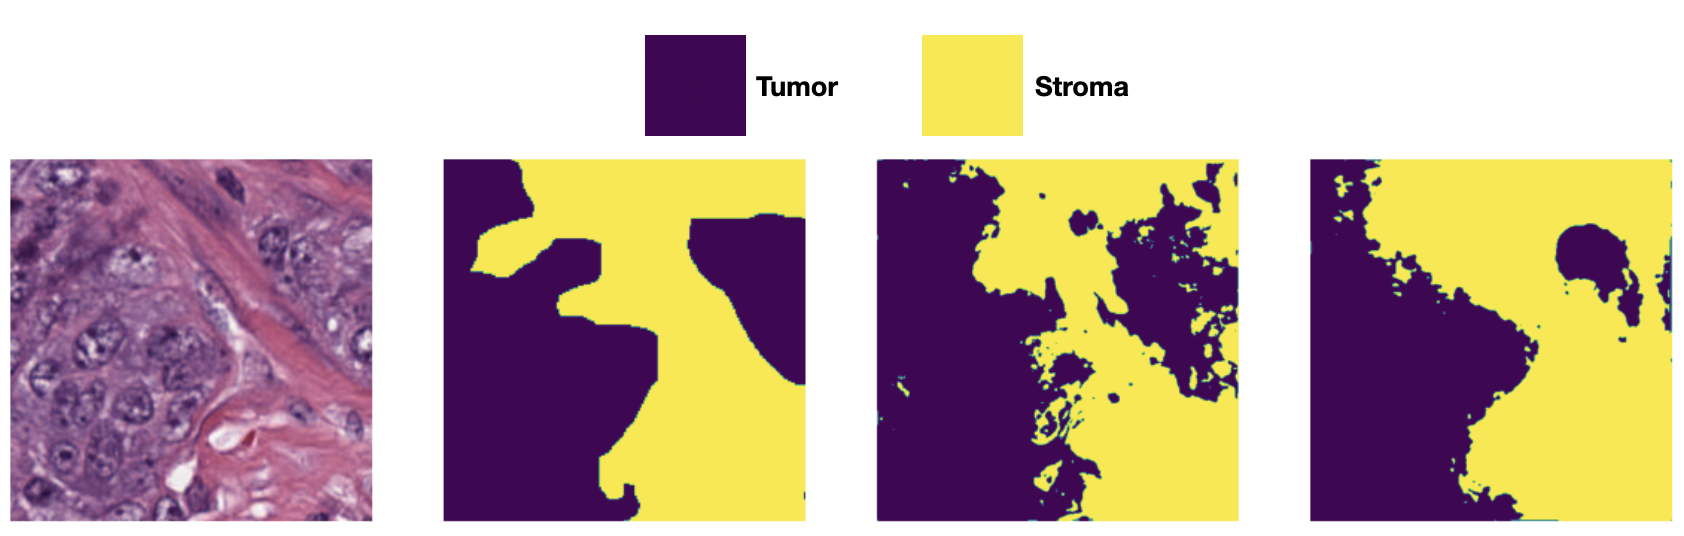
\includegraphics[width=0.9\linewidth]{media/Compare.png}
\end{center}
   \caption{Segmentation Results (From left to right): WSI, Ground Truth, UNet, UNet-MV2}
\label{fig:seg}
% \label{fig:onecol}
\end{figure}

\begin{table}[ht]
\centering
\begin{tabularx}{\columnwidth}{ >{\centering\arraybackslash}X | >{\centering\arraybackslash}X | >{\centering\arraybackslash}X }
\toprule
Works & Pixel Accuracy & Training Time \newline (minutes) \\
\midrule
UNet \cite{ronneberger2015unet}    & 0.67  & 13 \\
UNet-MV2 & 0.76 & 16 \\
TransUNet \cite{chen2021transunet} & 0.63 & 63\\
\bottomrule
\end{tabularx}
\caption{Comparison of pixel accuracy and average training time per epoch for state-of-the-art models}
\label{seg}
\end{table}

Due to the computation cost of the baseline approaches, we plan to apply patches based approach which consist of training with input size $(128\times 128)$ and perform inference with images of size $(512\times 512)$ by iterating over patches with recombination after prediction. Same as in classification, we will include the evaluation metric results with computational details in our final report. 

\section{Conclusion}
In this stage of work we proposed a classification model that achieved a reasonable performance over existing methods. Some baseline models were explored for segmentation tasks. Some evaluation metrics need to be integerated in the upcoming segmentation experiments, which is underway. Moreover, some preliminary experiments with simple upsampling head for segmenetation were not as successful, hence some better architectures should be considered. If time permits, creating a stronger image representation with Transformer architecture would be interesting. Contrastive learning has shown promises in producing a more robust encodings for downstream tasks. 

% \section{Conclusion}
% In this stage of work  we proposed a classification model for histological images using ViT architecture. The proposed method is fast to train and achieved good performance compared to previous works. In the coming stage, we will evaluate the model performance using the proposed metrics. Also, we will conduct more classification experiments to include the multi classes classification results. After that we will apply the proposed architecture for WSI segmentation. Finally we will investigate transfer learning and domain adaptation.

{\small
\bibliographystyle{ieee_fullname}
\bibliography{reference}}

\end{document}
